% !TEX root = saveliev_physics_general_course_2.tex
%!TEX TS-program = pdflatex
%!TEX encoding = UTF-8 Unicode


\chapter[ELECTRICAL OSCILLATIONS]{ELECTRICAL OSCILLATIONS}\label{chap:13}
\chaptermark{ELECTRICAL OSCILLATIONS}

\section{Quasistationary Currents}\label{sec:13_1}

When considering electrical oscillations, we have to do with time-varying currents.
Ohm's law and Kirchhoff's rules following from it were established for a steady current.
They also hold, however, for the instantaneous values of a varying current and voltage if the changes are not too fast.
Electromagnetic disturbances propagate along a circuit with a tremendous speed equal to the speed of light $c$.
Assume that the length of a circuit is $l$.
If during the time $\tau=l/c$ needed for the transmission of a disturbance to the farthest point of a circuit, the current changes insignificantly, then the instantaneous values of the current in all the cross sections of the circuit will be virtually identical.
Currents obeying this condition are called \textbf{quasistationary}.
For periodically varying currents, the condition for a
quasistationary state is
\begin{equation*}
    \tau = \frac{l}{c} \ll T,
\end{equation*}

\noindent
where $T$ is the period of the changes.

The delay for a circuit \SI{3}{\metre} long is $\tau=\SI{e-8}{\second}$.
Thus, up to values of $T$ of the order of \SI{e-6}{\second} (which corresponds to a frequency of \SI{e6}{\hertz}), the currents in such a circuit may be considered quasistationary.
A current of industrial frequency ($\nu= 50$ or \SI{60}{\hertz}) is quasistationary for circuits up to about \SI{100}{\kilo\metre} long.

The instantaneous values of quasistationary currents obey Ohm's law.
Hence, Kirchhoff's rules also hold for them.

In the following when studying electrical oscillations, we shall always assume that the currents we are dealing with are quasistationary.

\section{Free Oscillations in a Circuit Without a Resistance}\label{sec:13_2}

Electrical oscillations may appear in a circuit containing an inductance and a capacitance.
Such a circuit is therefore called an \textbf{oscillatory circuit}.
Figure \ref{fig:13_1}a shows the consecutive stages of an oscillatory process in an idealized circuit containing no resistance.

\begin{figure}[t]
	\begin{center}
		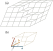
\includegraphics[scale=1.1]{figures/ch_13/fig_13_1.pdf}
		\caption[]{}
		\label{fig:13_1}
	\end{center}
	\vspace{-0.8cm}
\end{figure}

Oscillations can be set up in the circuit either by supplying a certain initial charge to the capacitor plates or by producing a current in the inductance (for example, by switching off the external magnetic field passing through the coil turns).
Let us use the first method.
We shall connect the capacitor to a source of voltage after disconnecting it from the inductance.
The result will be the appearance of unlike charges $+q$ and $-q$ on the plates (stage $1$).
An electric field will be set up between the plates, and its energy will be $(q^2/C)/2$ [see \eqn{4_5}].
If we next switch off the voltage source and connect the capacitor to the inductance, it will begin to discharge, and a current will flow through the circuit.
The energy of the electric field will diminish as a result, but in return a constantly growing energy of the magnetic field set up by the current flowing through the inductance will appear.
This energy is $LI^2/2$ [see \eqn{8_37}].

Since the resistance of the circuit is zero, the total energy consisting of the energies of the electric and magnetic fields is not used for heating the wires and will remain constant\footnote{Strictly speaking, in such an idealized circuit, energy would be lost on the radiation of electromagnetic waves. This loss grows with an increasing frequency of oscillations and when the circuit is more ``open''.}.
Therefore, at the moment when the voltage across the capacitor and, consequently, the energy of the electric field, vanish, the energy of the magnetic field and, consequently, the current reach their maximum value (stage $2$; beginning from this moment, the current flows at the expense of the self induced e.m.f.).
After this, the current diminishes, and, when the charges on the plates reach their initial value $q$, the current will vanish (stage $3$).
Next, the same processes occur in the opposite direction (stages $4$ and $5$).
After them, the system returns to its initial state (stage $5$), and the entire cycle repeats again and again.
The charge on the plates, the voltage across the capacitor, and the current flowing in the inductance periodically change (\ie, oscillate) during the process.
The oscillations are attended by mutual transformations of the electric and magnetic field energies.

Figure \ref{fig:13_1}b compares the oscillations of a
spring pendulum with those in the circuit.
The supply of charges to the capacitor plates corresponds to bringing the pendulum out of its equilibrium position by exerting an external force on it and imparting the initial deviation $x$ to it.
The potential energy of elastic deformation of the spring equal to $kx^2/2$ is produced.
Stage $2$ corresponds to passing of the pendulum through its equilibrium position.
At this moment, the quasi-elastic force vanishes, and the pendulum continues its motion by inertia.
By this time, the energy of the pendulum completely transforms into kinetic energy and is determined by the expression $mx^2/2$.
We shall let our reader compare the further stages.

It can be seen from a comparison of electrical and mechanical oscillations that the energy of an electric field $(q^2/C)/E$ is similar to the potential energy of elastic deformation, and the energy of a magnetic field $LI^2/2$ is similar to the kinetic energy.
The inductance $L$ plays the part of the mass $m$, and the reciprocal of the capacitance $(1/C)$ the part of the spring constant $k$.
Finally, the displacement $x$ of the pendulum from its equilibrium position corresponds to the charge $q$, and the speed $\dot{x}$ to the current $I = \dot{q}$.
We shall see below that the analogy between electrical and mechanical oscillations also extends to the mathematical equations describing them.

Let us find an equation for the oscillations in a circuit without a resistance (an $L$-$C$ circuit).
We shall consider the current charging the capacitor to be positive\footnote{With such a choice of the direction of the current, the analogy between electrical and mechanical oscillations is more complete: $\dot{q}$ corresponds to the speed $\dot{X}$ (with a different choice, $-\dot{q}$ corresponds to the speed $\dot{x}$).} (\fig{13_2}).
Hence, by \eqn{5_1},
\begin{equation*}
    I = \diff{q}{t} = \dot{q}.
\end{equation*}

\begin{figure}[t]
	\begin{center}
		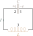
\includegraphics[scale=1]{figures/ch_13/fig_13_2.pdf}
		\caption[]{}
		\label{fig:13_2}
	\end{center}
	\vspace{-0.8cm}
\end{figure}

\noindent
Equation \eqref{eq:5_27} of Ohm's law for circuit $1$-$3$-$2$ is
\begin{equation*}
    IR = \varphi_1 - \varphi_2 + \mathcal{E}_{12}.
\end{equation*}

\noindent
In our case, $R=0$, $\varphi_1 - \varphi_2=-q/C$, and $\mathcal{E}_{12}=\ab{\mathcal{E}}{s} = -L\, (\diffin{I}{t})$.
Introducing these values into \eqn{5_27}, we get
\begin{equation}\label{eq:13_1}
    0 = - \frac{q}{C} - L\, \diff{I}{t}.
\end{equation}

\noindent
Finally, replacing $\diffin{I}{t}$ with $\ddot{q}$ [see \eqn{5_1}], we get
\begin{equation}\label{eq:13_2}
    \ddot{q} + \frac{1}{LC} q = 0.
\end{equation}

If we introduce the symbol
\begin{equation}\label{eq:13_3}
    \omega_0 = \frac{1}{\sqrt{LC}},
\end{equation}

\noindent
\eqn{13_2} becomes
\begin{equation}\label{eq:13_4}
    \ddot{q} + \omega_0^2 q = 0,
\end{equation}

\noindent
which is our good acquaintance from the science of mechanical oscillations [see Eq. (7.7) of Vol. I].
The following function is a solution of this equation:
\begin{equation}\label{eq:13_5}
    q = \ab{q}{m} \cos(\omega_0 t + \alpha)
\end{equation}

\noindent
(the subscript ``m'' stands for maximum).

Thus, the charge on the capacitor plates changes according to a harmonic law with a frequency determined by \eqn{13_3}.
This frequency is called the \textbf{natural frequency of the circuit} (it corresponds to the natural frequency of a harmonic oscillator).
We get the so-called \textbf{Thomson formula} for the period of the oscillations:
\begin{equation}\label{eq:13_6}
    T = \frac{2\pi}{\sqrt{LC}}.
\end{equation}

The voltage across the capacitor differs from the charge by the factor $1/C$:
\begin{equation}\label{eq:13_7}
    U = \frac{\ab{q}{m}}{C} \cos(\omega_0 t + \alpha) = \ab{U}{m} \cos(\omega_0 t + \alpha).
\end{equation}

Time differentiation of \eqn{13_5} yields an expression for the current:
\begin{equation}\label{eq:13_8}
    I = - \omega_0 \ab{q}{m} \sin(\omega_0 t + \alpha) = \ab{I}{m} \cos(\omega_0 t + \alpha + \frac{\pi}{2}).
\end{equation}

\noindent
Thus, the current leads the voltage across the capacitor in phase by $\pi/2$.

A comparison of \eqns{13_5}{13_7} with \eqn{13_8} shows that at the moment when the current reaches its maximum value, the charge and the voltage vanish, and vice versa.
We have already established this relation between the charge and the current on the basis of energy considerations.

Examination of \eqns{13_7}{13_8} shows that
\begin{equation*}
    \ab{U}{m} = \frac{\ab{q}{m}}{C}, \quad \ab{I}{m} = \omega_0 \ab{q}{m}.
\end{equation*}

\noindent
Taking the ratio of these amplitudes and substituting for $\omega_0$ its value from \eqn{13_3}, we get
\begin{equation}\label{eq:13_9}
    \ab{U}{m} = \parenthesis{\frac{L}{C}}^{1/2}\, \ab{I}{m}.
\end{equation}

\noindent
We can also obtain this equation if we proceed from the fact that the maximum value of the energy of the electric field $C\ab{U}{m}^2/2$ must equal the maximum value of the energy of the magnetic field $L\ab{I}{m}^2/2$.

\section{Free Damped Oscillations}\label{sec:13_3}

Any real circuit has a resistance.
The energy stored in the circuit is gradually spent in this resistance for heating, owing to which the free oscillations become damped.
Equation \eqref{eq:5_27} written for circuit $1$-$3$-$2$ shown in \fig{13_3} has the form
\begin{equation}\label{eq:13_10}
    IR = - \frac{q}{C} - L\, \diff{I}{t}
\end{equation}

[compare with \eqn{13_1}].
Dividing this equation by $L$ and substituting $\dot{q}$ for $I$ and $\ddot{q}$ for $\diffin{I}{t}$, we obtain
\begin{equation}\label{eq:13_11}
    \ddot{q} + \frac{R}{L}\, \dot{q} + \frac{1}{LC}\, q = 0.
\end{equation}

\begin{figure}[t]
	\begin{center}
		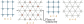
\includegraphics[scale=1]{figures/ch_13/fig_13_3.pdf}
		\caption[]{}
		\label{fig:13_3}
	\end{center}
	\vspace{-0.8cm}
\end{figure}

Taking into account that the reciprocal of $LC$ equals the square of the natural frequency of the circuit $\omega_0$ [see \eqn{13_3}], and introducing
the symbol
\begin{equation}\label{eq:13_12}
    \beta = \frac{R}{LC},
\end{equation}

\noindent
\eqn{13_11} can be written in the form
\begin{equation}\label{eq:13_13}
    \ddot{q} + 2 \beta \dot{q} + \omega_0^2 q = 0.
\end{equation}

This equation coincides with the differential equation of damped mechanical oscillations [see Eq. (7.11) of Vol. I].

When $\beta^2<\omega_0^2$, \ie, $R^2/(4L^2)<1/(LC)$, the solution of \eqn{13_3} has the form
\begin{equation}\label{eq:13_14}
    q = \ab{q}{m,$0$}\, e^{-\beta t} \cos(\omega t + \alpha),
\end{equation}

\noindent
where $\omega=\sqrt{\omega_0^2-\beta^2}$.
Substituting for $\omega_0$ its value from \eqn{13_3} and for $\beta$ its value from \eqn{13_12}, we find that
\begin{equation}\label{eq:13_15}
    \omega = \parenthesis{ \frac{1}{LC} - \frac{R^2}{4L^2} }.
\end{equation}

\noindent
Thus, the frequency of damped oscillations $\omega$ is smaller than the natural frequency $\omega_0$.
When $R=0$, \eqn{13_13} transforms into \eqn{13_3}.

Dividing \eqn{13_14} by the capacitance $C$, we get the voltage across the capacitor:
\begin{equation}\label{eq:13_16}
    U = \frac{1}{C} \ab{q}{m,$0$}\, e^{-\beta t} \cos(\omega t + \alpha) = \ab{U}{m,$0$}\, e^{-\beta t} \cos(\omega t + \alpha).
\end{equation}

To find the current, we shall differentiate \eqn{13_14} with respect to time
\begin{equation*}
    I = \dot{q} = \ab{q}{m,$0$}\, e^{-\beta t} [-\beta \cos(\omega t + \alpha) - \omega \sin(\omega t + \alpha)].
\end{equation*}

\noindent
Multiplying the right-hand side of this equation by the expression
\begin{equation*}
    \frac{\omega_0}{\sqrt{\omega^2-\beta^2}}
\end{equation*}

\noindent
equal to unity, we get
\begin{equation*}
    I = \omega_0 \ab{q}{m,$0$}\, e^{-\beta t} \bracket{ - \frac{\beta}{\sqrt{\omega^2-\beta^2}} \cos(\omega t + \alpha) - \frac{\omega}{\sqrt{\omega^2-\beta^2}} \sin(\omega t + \alpha) }.
\end{equation*}

Introducing the angle $\psi$ determined by the conditions
\begin{equation*}
    \cos\psi = - \frac{\beta}{\sqrt{\omega^2-\beta^2}} = - \frac{\beta}{\omega_0},\quad \sin\psi = \frac{\omega}{\sqrt{\omega^2-\beta^2}} = \frac{\omega}{\omega_0},
\end{equation*}

\noindent
we can write
\begin{equation}\label{eq:13_17}
    I = \omega_0 \ab{q}{m,$0$}\, e^{-\beta t} \cos(\omega t + \alpha + \psi).
\end{equation}

\noindent
Since $\cos\psi<0$ and $\sin\psi>0$, the value of $\psi$ is within the limits from $\pi/2$ to $\pi$ (\ie, $\pi/2<\psi<\pi$).
Thus, when a circuit contains a resistance, the current leads the voltage across the capacitor in phase by more than $\pi/2$ (when $R=0$, the advance in phase is $\pi/2$).

A plot of function \eqref{eq:13_14} is depicted in \fig{13_4}.
Plots of the voltage and current are similar to it.

It is customary practice to characterize the damping of oscillations by the \textbf{logarithmic decrement}
\begin{equation}\label{eq:13_18}
    \lambda = \ln\bracket{ \frac{A(t)}{A(t+T)} } = \beta T
\end{equation}

\noindent
[see Eq. (7.104) of Vol. I].
Here $A(t)$ is the amplitude of the relevant quantity ($q$, $U$, or $I$).
We remind our reader that the logarithmic decrement is the reciprocal of the number of oscillations $N_e$ performed during the time needed for the amplitude to decrease to $1/e$ of its initial value:
\begin{equation*}
    \lambda = \frac{1}{N_e}.
\end{equation*}

\begin{figure}[t]
	\begin{center}
		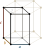
\includegraphics[scale=1]{figures/ch_13/fig_13_4.pdf}
		\caption[]{}
		\label{fig:13_4}
	\end{center}
	\vspace{-0.8cm}
\end{figure}

Using in \eqn{13_18} the value of $\beta$ from \eqn{13_12} and substituting $2\pi/\omega$ for $T$, we get the following expression for $A$:
\begin{equation}\label{eq:13_19}
    \lambda = \frac{R}{2L} \frac{2\pi}{\omega} = \frac{\pi R}{L\omega}.
\end{equation}

\noindent
The frequency $\omega$, and, therefore, also $A$ are determined by the parameters of a circuit $L$, $C$, and $R$.
Thus, the logarithmic decrement is a characteristic of a circuit.

If the damping is not great ($\beta^2\ll\omega_0^2$), we can assume in \eqn{13_19} that $\omega\approx\omega_0 = 1/\sqrt{LC}$.
Hence,
\begin{equation}\label{eq:13_20}
    \lambda \approx \frac{\pi R \sqrt{LC}}{L} = \pi R \parenthesis{\frac{C}{L}}^{1/2}.
\end{equation}

An oscillatory circuit is often characterized by its quality, or simply $Q$, determined as a quantity that is inversely proportional to the logarithmic decrement:
\vspace{-12pt}
\begin{equation}\label{eq:13_21}
    Q = \frac{\pi}{\lambda} = \pi N_e.
\end{equation}

\noindent
It follows from \eqn{13_21} that the quality of a circuit is the higher, the greater is the number of oscillations completed before the amplitude diminishes to $1/e$ of its initial value.

For weak damping, we have
\begin{equation}\label{eq:13_22}
    Q = \frac{1}{R} \parenthesis{\frac{L}{C}}^{1/2}
\end{equation}

\noindent
[see \eqn{13_20}].

In Sec. 7.10 of Vol. I, we showed that when the damping is weak, the quality of a mechanical oscillatory system equals the ratio of the energy stored in the system at a given moment to the decrement of this energy during one period of oscillations with an accuracy to the factor $2\pi$.
We shall show that this also holds for electrical oscillations.
The amplitude of the current in a circuit diminishes according to the law $e^{-\beta t}$.
The energy $W$ stored in the circuit is proportional to the square of the current amplitude (or to the square of the amplitude of the voltage across the capacitor).
Hence, $W$ diminishes according to the law $e^{-2\beta t}$.
The relative reduction in the energy during a period is
\begin{equation*}
    \frac{\Delta{W}}{W} = \frac{W(t) - W(t+T)}{W(t)} = \frac{1 - e^{-2\beta t}}{1} = 1 - e^{-2\lambda}.
\end{equation*}

\noindent
With insignificant damping (\ie, when $A\ll 1$), we may assume that $e^{-2\lambda}$ is approximately equal to $1-2\lambda$:
\begin{equation*}
    \frac{\Delta{W}}{W} = 1 - (1 - 2\lambda) = 2 \lambda.
\end{equation*}

\noindent
Finally, substituting the quality $Q$ of the circuit for $\lambda$ in this expression in accordance with \eqn{13_21} and solving the equation obtained relative to $Q$, we get
\begin{equation}\label{eq:13_23}
    Q = 2\pi \frac{\Delta{W}}{W}.
\end{equation}

We shall note in conclusion that when $R^2/(4L^2)\geqslant 1/(LC)$, \ie, when $\beta^2\geqslant\omega_0^2$, an aperiodic discharge of the capacitor occurs instead of oscillations.
The resistance of a circuit at which an oscillatory process transforms into an aperiodic one is called \textbf{critical}.
The value of the critical resistance $\ab{R}{cr}$ is determined by the condition $\ab{R}{cr}^2/(4L^2)= 1/(LC)$, whence
\begin{equation}\label{eq:13_24}
    \ab{R}{cr} = 2 \parenthesis{\frac{L}{C}}^{1/2}.
\end{equation}

\section{Forced Electrical Oscillations}\label{sec:13_4}

To produce forced oscillations of a system, an external periodically changing action must be exerted on it.
This can be achieved for electrical oscillations if we connect a varying e.m.f. in series with the circuit elements or, if after breaking the circuit, we feed an alternating voltage to the contacts formed, \ie, the voltage
\begin{equation}\label{eq:13_25}
    U = \ab{U}{m} \cos(\omega t)
\end{equation}

\noindent
(\fig{13_5}).
This voltage must be added to the self-induced e.m.f..
As a result, \eqn{13_10} acquires the form
\begin{equation}\label{eq:13_26}
    IR = - \frac{q}{C} - L\, \diff{I}{t} + \ab{U}{m} \cos(\omega t).
\end{equation}

\noindent
After transformations, we get the equation
\begin{equation}\label{eq:13_27}
    \ddot{q} + 2\beta \dot{q} + \omega_0^2 q = \frac{\ab{U}{m}}{L} \cos(\omega t).
\end{equation}

\noindent
Here, $\omega_0^2$ and $\beta$ are determined by \eqns{13_3}{13_12}.

\begin{figure}[t]
	\begin{center}
		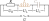
\includegraphics[scale=1]{figures/ch_13/fig_13_5.pdf}
		\caption[]{}
		\label{fig:13_5}
	\end{center}
	\vspace{-0.8cm}
\end{figure}

Equation \eqref{eq:13_27} coincides with the differential equation of forced mechanical oscillations [see Eq. (7.111) of Vol. I].
A partial solution of this equation has the form
\begin{equation}\label{eq:13_28}
    q = \ab{q}{m} \cos(\omega t - \psi),
\end{equation}

\noindent
where
\begin{equation*}
    \ab{q}{m} = \frac{\ab{U}{m}/L}{\sqrt{\parenthesis{\omega_0^2-\omega^2}^2 + 4\beta^2\omega^2}},\quad \tan\psi = \frac{2\beta\omega}{\omega_0^2-\omega^2}
\end{equation*}

\noindent
[see Eq. (7.119) of Vol. I].
Substitution of their values for $\omega_0$ and $\beta$ gives
\begin{align}
    \ab{q}{m} &= \frac{\ab{U}{m}}{\omega \sqrt{R^2 + [\omega L - 1/(\omega C)]^2}},\label{eq:13_29}\\
    \tan\psi &= \frac{R}{[1/(\omega C) - \omega L]}.\label{eq:13_30}
\end{align}

A general solution is obtained if we add the general solution of the relevant homogeneous equation to partial solution \eqref{eq:13_28}.
This solution was obtained in the preceding section [see \eqn{13_14}].
It contains the exponential factor $e^{-\beta t}$, therefore, after sufficient time elapses, becomes very small and it may be disregarded.
Consequently, stationary forced oscillations are described by the function \eqref{eq:13_28}.

Time differentiation of \eqn{13_28} gives the current in a circuit with stationary oscillations:
\begin{equation*}
    I = -\omega \ab{q}{m} \sin(\omega t - \psi) = \ab{I}{m} \cos\parenthesis{ \omega t - \psi + \frac{\pi}{2} }
\end{equation*}

\noindent
($\ab{I}{m}=\omega\ab{q}{m}$).
Let us write this expression in the form\footnote{We shall not encounter the concept of potential any more up to the end of this chapter. Therefore, no misunderstandings will appear if we use the symbol $\varphi$ for the phase angle.}
\begin{equation}\label{eq:13_31}
    I = \ab{I}{m} \cos(\omega t - \varphi),
\end{equation}

\noindent
where $\varphi=\psi-\pi/2$ is the shift in phase between the current and the applied voltage [see \eqn{13_25}].
In accordance with \eqn{13_30}:
\begin{equation}\label{eq:13_32}
    \tan\varphi = \tan\parenthesis{\psi - \frac{\pi}{2}} = - \frac{q}{\tan\psi} = \frac{\omega L - 1/(LC)}{R}.
\end{equation}

\noindent
Inspection of this equation shows that the current lags in phase behind the voltage ($\varphi>0$) when $\omega L>1/(\omega C)$, and leads the voltage ($\varphi<0$) when $\omega L<1/(\omega C)$.
According to \eqn{13_29}:
\begin{equation}\label{eq:13_33}
    \ab{I}{m} = \omega \ab{q}{m} = \frac{\ab{U}{m}}{\sqrt{R^2 + [\omega L - 1/(\omega C)]^2}}.
\end{equation}

\noindent
Let us write \eqn{13_26} in the form
\begin{equation}\label{eq:13_34}
    IR + \frac{q}{C} + L\, \diff{I}{t} = \ab{U}{m} \cos(\omega t).
\end{equation}

\noindent
The product $IR$ equals the voltage $U_R$ across the resistance, $q/C$ is the voltage across the capacitor $U_C$, and the expression $L\,(\diffin{I}{t})$ determines the voltage across the inductance $U_L$.
Taking this into account, we can write
\begin{equation}\label{eq:13_35}
    U_R + U_C + U_L = \ab{U}{m} \cos(\omega t).
\end{equation}

\noindent
Thus, the sum of the voltages across the separate elements of a circuit at each moment of time equals the voltage applied from an external source (see \fig{13_5}).

According to \eqn{13_31}
\begin{equation}\label{eq:13_36}
    U_R = R \ab{I}{m} \cos(\omega t - \varphi).
\end{equation}

\noindent
Dividing \eqn{13_28} by the capacitance, we get the voltage across the capacitor
\begin{equation}\label{eq:13_37}
    U_C = \frac{\ab{q}{m}}{C} \cos(\omega t - \psi) = \ab{U}{$C$,m} \cos\parenthesis{\omega t - \varphi - \frac{\pi}{2}}.
\end{equation}

\noindent
Here,
\begin{equation}\label{eq:13_38}
    \ab{U}{$C$,m} = \frac{\ab{q}{m}}{C}  = \frac{\ab{U}{m}}{\omega C \sqrt{R^2 + [\omega L - 1/(\omega C)]^2}} = \frac{\ab{I}{m}}{\omega C}
\end{equation}

\noindent
[see \eqn{13_31}].
Multiplying the derivative of function \eqref{eq:13_31} by $L$, we get the voltage across the inductance:
\begin{equation}\label{eq:13_39}
    U_L = L\, \diff{I}{t} = - \omega L \ab{I}{m} \sin(\omega t - \varphi) = \ab{U}{$L$,m} \cos\parenthesis{\omega t - \varphi + \frac{\pi}{2}}.
\end{equation}

\noindent
Here,
\begin{equation}\label{eq:13_40}
    \ab{U}{$L$,m} = \omega L \ab{I}{m}.
\end{equation}

A comparison of Eqs. \eqref{eq:13_31}, \eqref{eq:13_36}, \eqref{eq:13_37}, and \eqref{eq:13_39} shows that the voltage across the capacitor lags in phase behind the current by $\pi/2$, while the voltage across the inductance leads the current by $\pi/2$.
The voltage across the resistance changes in phase with the current.
The phase relations can be shown very clearly with the aid of a vector diagram (see Sec. 7.7 of Vol. I).
We remind our reader that a harmonic oscillation (or a harmonic function) can be shown with the aid of a vector whose length equals the amplitude of the oscillation, while the direction of the vector makes an angle equal to the initial phase of the oscillation with a certain axis.
Let us take the axis of currents as the straight line from which the initial phase is counted.
This gives us the diagram shown in \fig{13_6}.

\begin{figure}[t]
	\begin{center}
		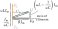
\includegraphics[scale=1]{figures/ch_13/fig_13_6.pdf}
		\caption[]{}
		\label{fig:13_6}
	\end{center}
	\vspace{-0.8cm}
\end{figure}

\noindent
According to \eqn{13_35}, the sum of the three functions $U_R$, $U_C$, and $U_L$ must equal the applied voltage $U$.
The voltage $U$ is accordingly shown in the diagram by a vector equal to the sum of the vectors $U_R$, $U_C$, and $U_L$.
We must note that \eqn{13_33} is easily obtained from the right triangle formed in the vector diagram by the vectors $U$, $U_R$, and the difference $U_L-U_C$.

The resonance frequency for the charge $q$ and the voltage $U_C$ across the capacitor is
\begin{equation}\label{eq:13_41}
    \ab{\omega}{$q$,res} = \ab{\omega}{$U$,res} = \parenthesis{\omega_0^2 - 2\beta^2}^{1/2} = \parenthesis{\frac{1}{LC} - \frac{R^2}{2L^2}}^{1/2}\leqslant \omega_0
\end{equation}

\noindent
[see Eq. (7.127) of Vol. I].

Resonance curves for $U_C$ are shown in \fig{13_7} (resonance curves for $q$ have the same form).
They are similar to the resonance curves obtained for mechanical oscillations (see Fig. 7.24 of Vol. I).
When $\omega\to 0$, the resonance curves converge at one point having the ordinate $\ab{U}{$C$,m}=\ab{U}{m}$, \ie, the voltage appearing across the capacitor when it is connected to a source of steady voltage $\ab{U}{m}$.
The maximum in resonance will be the higher and the sharper, the smaller is $\beta=R/(2L)$, \ie, the smaller is the resistance and the greater the inductance of the circuit.

Resonance curves for the current are shown in \fig{13_8}.
They correspond to the resonance curves for the velocity in mechanical oscillations.
The amplitude of the current has a maximum value at
$\omega L - 1/(\omega C)$ [see \eqn{13_33}]. Consequently, the resonance frequency for the current coincides with the natural frequency of the circuit $\omega_0$:
\begin{equation}\label{eq:13_42}
    \ab{\omega}{$I$,res} = \omega_0 = \frac{1}{\sqrt{LC}}.
\end{equation}

\begin{figure}[t]
	\begin{minipage}[t]{0.48\linewidth}
		\begin{center}
			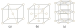
\includegraphics[scale=1]{figures/ch_13/fig_13_7.pdf}
			\caption[]{}
			\label{fig:13_7}
		\end{center}
	\end{minipage}
	\hfill{ }%space{-0.05cm}
	\begin{minipage}[t]{0.48\linewidth}
		\begin{center}
			
\includegraphics[scale=1]{figures/ch_13/fig_13_8.pdf}
			\caption[]{}
			\label{fig:13_8}
		\end{center}
	\end{minipage}
\vspace{-0.4cm}
\end{figure}

The intercept formed by the resonance curves on the $\ab{I}{m}$-axis is zero---at a constant voltage, a steady current cannot flow in a circuit containing a capacitor.

At small damping (when $\beta^2\ll\omega_0^2$), the resonance frequency for the voltage can be taken equal to $\omega_0$ [see \eqn{13_41}].
Accordingly, we may consider that $\ab{\omega}{res}L-1/(\ab{\omega}{res}C)$.
By \eqn{13_38}, the ratio of the amplitude of the voltage across the capacitor in resonance $\ab{U}{$C$,m,res}$ to the amplitude of the external voltage $\ab{U}{m}$ will in this case be
\begin{equation}\label{eq:13_43}
    \frac{\ab{U}{$C$,m,res}}{\ab{U}{m}} = \frac{1}{\omega_0 CR} = \frac{\sqrt{LC}}{CR} = \frac{1}{R} \parenthesis{\frac{L}{C}}^{1/2} = Q
\end{equation}

\noindent
[we have assumed in \eqn{13_38} that $\omega=\ab{\omega}{$U$,res}=\omega_0$.
Here, $Q$ is the quality of the circuit [see \eqn{13_22}].
Thus, the quality of a circuit shows how many times the voltage across a capacitor can exceed the applied voltage.

The quality of a circuit also determines the sharpness of the resonance curves.
Figure \ref{fig:13_9} shows a resonance curve for the
current in a circuit.
Instead of laying off the values of $\ab{I}{m}$ corresponding to a given frequency along the axis of ordinates, we have laid off the ratio of $\ab{I}{m}$ to $\ab{I}{m,res}$ (\ie, to $\ab{I}{m}$ in resonance).
Let us consider the width of the curve $\Delta{\omega}$ taken at the height $0.7$ (a power ratio of $0.7^2\approx 0.5$ corresponds to a ratio of the current amplitudes equal to $0.7$).
We can show that the ratio of this width to the resonance frequency equals a quantity that is the reciprocal of the quality of a circuit:
\begin{equation}\label{eq:13_44}
    \frac{\Delta{\omega}}{\omega_0} = \frac{1}{Q}.
\end{equation}

\begin{figure}[t]
	\begin{center}
		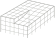
\includegraphics[scale=1]{figures/ch_13/fig_13_9.pdf}
		\caption[]{}
		\label{fig:13_9}
	\end{center}
	\vspace{-0.8cm}
\end{figure}

We remind our reader that \eqns{13_43}{13_44} hold only for large values of $Q$, \ie, when the damping of the free oscillations in the circuit is small.

The phenomenon of resonance is used to separate the required component from a complex voltage.
Assume that the voltage applied to a circuit is
\begin{equation*}
    U = \ab{U}{m,$1$} \cos(\omega_1 t + \alpha_1) + \ab{U}{m,$2$} \cos(\omega_2 t + \alpha_2) + \ldots.
\end{equation*}

\noindent
By tuning the circuit to one of the frequencies $\omega_1$, $\omega_2$, etc. (\ie, by correspondingly choosing its parameters $C$ and $L$), we can obtain a voltage across the capacitor that exceeds the value of the given component $Q$ times, whereas the voltage produced across the capacitor by the other components will be weak.
Such a process is carried out, for example, when tuning a radio receiver to the required wavelength.

\section{Alternating Current}\label{sec:13_5}

The stationary forced oscillations described in the preceding section can be considered as the flow of an alternating current produced by the alternating voltage
\vspace{-12pt}
\begin{equation}\label{eq:13_45}
    U = \ab{U}{m} \cos(\omega t)
\end{equation}

\noindent
in a circuit including a capacitance, an inductance, and a resistance.
According to Eqs. \eqref{eq:13_31}, \eqref{eq:13_32}, and \eqref{eq:13_33}, this current varies according to the law
\begin{equation}\label{eq:13_46}
    I = \ab{I}{m} \cos(\omega t - \varphi).
\end{equation}

\noindent
The amplitude of the current is determined by the amplitude of the voltage $\ab{U}{m}$ the circuit parameters $C$, $L$, $R$, and the frequency $\omega$:
\begin{equation}\label{eq:13_47}
    \ab{I}{m} = \frac{\ab{U}{m}}{\sqrt{R^2+[\omega L - 1/(\omega C)]^2}}.
\end{equation}

\noindent
The current lags in phase behind the voltage by the angle $\varphi$ that depends on the parameters of the circuit and on the frequency:
\begin{equation}\label{eq:13_48}
    \tan\varphi = \frac{\omega L - 1/(\omega C)}{R}.
\end{equation}

\noindent
When $\varphi<0$, the current actually leads the voltage.

The expression
\begin{equation}\label{eq:13_49}
    Z = \parenthesis{R^2 + \parenthesis{\omega L - \frac{1}{\omega C}}^2}^{1/2}
\end{equation}

\noindent
in the denominator of \eqn{13_47} is called the \textbf{impedance}.

If a circuit consists only of a resistance $R$, the equation of Ohm's law has the form
\begin{equation*}
    IR = \ab{U}{m} \cos(\omega t).
\end{equation*}

\noindent
Hence, it follows that the current in this case varies in phase with the voltage, while the amplitude of the current is
\begin{equation*}
    \ab{I}{m} = \frac{\ab{U}{m}}{R}.
\end{equation*}

\noindent
A comparison of this expression with \eqn{13_47} shows that the replacement of a capacitor with a shorted circuit section signifies a transition to $C\to\infty$ instead of to $C=0$.

Any real circuit has finite values of $R$, $L$, and $C$.
It may happen that some of these parameters are such that their influence on the current may be disregarded.
Suppose that $R$ of a circuit may be assumed equal to zero, and $C$ equal to infinity.
Now, we can see from \eqns{13_47}{13_48} that
\begin{equation}\label{eq:13_50}
    \ab{I}{m} = \frac{\ab{U}{m}}{\omega L}
\end{equation}

\noindent
and that $\tan\varphi=\infty$ (accordingly, $\varphi=\pi/2$).
The quantity
\begin{equation}\label{eq:13_51}
    X_L = \omega L
\end{equation}

\noindent
is called the \textbf{inductive reactance}.
If $L$ is expressed in henries, and $\omega$ in \si{\radian\per\second}, then $X_L$ will be expressed in ohms.
Examination of \eqn{13_51} shows that the inductive reactance grows with the frequency $\omega$.
An inductance does not react to a steady current ($\omega=0$), \ie, $X_L=0$.

The current in an inductance lags behind the voltage by $\pi/2$.
Accordingly, the voltage across the inductance leads the current by $\pi/2$ (see \fig{13_6}).

Now, let us assume that $R$ and $L$ both equal zero.
Hence, according to \eqns{13_47}{13_48}, we have
\begin{equation}\label{eq:13_52}
    \ab{I}{m} = \frac{\ab{U}{m}}{1/(\omega C)}
\end{equation}

\noindent
$\tan\varphi=-\infty$ (\ie, $\varphi=-\pi/2$).
The quantity
\begin{equation}\label{eq:13_53}
    X_C = \frac{1}{\omega C}
\end{equation}

\noindent
is called the \textbf{capacitive reactance}.
If $C$ is expressed in farads, and $\omega$ in \si{\radian\per\second} then $X_C$ will be expressed in ohms.
It follows from \eqn{13_53} that the capacitive reactance diminishes with increasing frequency.
For a steady current, $X_C=\infty$---a steady current cannot flow through a capacitor.
Since $\varphi=-\pi/2$, the current flowing through a capacitor leads the voltage by $\pi/2$.
Accordingly, the voltage across a capacitor lags behind the current by $\pi/2$ (see \fig{13_6}).

Finally, suppose that we may assume $R$ to equal zero.
In this case, \eqn{13_47} becomes
\begin{equation}\label{eq:13_54}
    \ab{I}{m} = \frac{\ab{U}{m}}{|\omega L - 1/(\omega C)|}.
\end{equation}

\noindent
The quantity
\begin{equation}\label{eq:13_55}
    X = \omega L - \frac{1}{\omega C} = X_L - X_C
\end{equation}

\noindent
is called the \textbf{reactance}.

Equations \eqref{eq:13_48} and \eqref{eq:13_49} can be written in the form
\begin{equation*}
    \tan\varphi = \frac{X}{R},\quad Z = \sqrt{R^2+X^2}.
\end{equation*}

\noindent
Thus, if the values of the resistance $R$ and the reactance $X$ are laid off along the legs of a right triangle, then the length of the hypotenuse will numerically equal $Z$ (see \fig{13_6}).

Let us find the power liberated in an alternating current circuit.
The instantaneous value of the power equals the product of the instantaneous values of the voltage and current:
\begin{equation}\label{eq:13_56}
    P(t) = U(t)I(t) = \ab{U}{m} \cos(\omega t) \times \ab{I}{m} \cos(\omega t - \varphi).
\end{equation}

\noindent
Taking advantage of the formula
\begin{equation*}
    \cos\alpha\cos\beta = \frac{1}{2}\cos(\alpha-\beta) + \frac{1}{2} \cos(\alpha+\beta),
\end{equation*}

\noindent
we can write \eqn{13_56} in the form
\begin{equation}\label{eq:13_57}
    P(t) = \frac{1}{2} \ab{U}{m} \ab{I}{m} \cos\varphi + \frac{1}{2} \ab{U}{m} \ab{I}{m} \cos(2\omega t - \varphi).
\end{equation}

Of practical interest is the time-average value $P(t)$, which we shall denote simply by $P$.
Since the average value of $\cos(2\omega t - \varphi)$ is zero, we have
\begin{equation}\label{eq:13_58}
    P = \frac{\ab{U}{m} \ab{I}{m}}{2} \cos\varphi.
\end{equation}

\noindent
Inspection of \eqn{13_57} shows that the instantaneous power fluctuates about the average value with a frequency double that of the current (\fig{13_10}).

\begin{figure}[t]
	\begin{center}
		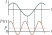
\includegraphics[scale=1]{figures/ch_13/fig_13_10.pdf}
		\caption[]{}
		\label{fig:13_10}
	\end{center}
	\vspace{-0.8cm}
\end{figure}

In accordance with \eqn{13_48},
\begin{equation}\label{eq:13_59}
    \cos\varphi = \frac{R}{\sqrt{R^2+[\omega L - 1/(\omega C)]^2}} = \frac{R}{Z}.
\end{equation}

\noindent
Using this value of $\cos\varphi$ in \eqn{13_48} and taking into account that $\ab{U}{m}/Z=\ab{I}{m}$, we get
\begin{equation}\label{eq:13_60}
    P = \frac{R\ab{I}{m}^2}{2}.
\end{equation}

\noindent
The same power is developed by a direct current whose strength is
\begin{equation}\label{eq:13_61}
    I = \frac{\ab{I}{m}}{\sqrt{2}}.
\end{equation}

\noindent
Quantity \eqref{eq:13_61} is known as the \textbf{effective value of the current}.
Similarly, the quantity
\begin{equation}\label{eq:13_62}
    U = \frac{\ab{U}{m}}{\sqrt{2}},
\end{equation}

\noindent
is called the \textbf{effective voltage}.

Expressing the average power through the effective current and voltage, we get
\begin{equation}\label{eq:13_63}
    P = U I \cos\varphi.
\end{equation}

\noindent
The factor $\cos\varphi$ in this expression is called the \textbf{power factor}.
Engineers try to make $\cos\varphi$ as high as possible.
At a low value of $\cos\varphi$, a large current must be passed through a circuit to obtain the required power, and this results in greater losses in the feeder lines.
